
Estas series permiten, en principio, la aproximación de funciones periódicas. Se examinan y representan funciones periódicas a través de su descomposición en una suma infinita de senos y cosenos con frecuencias enteras.

\section{Función periódica}

Una función periódica es una función $f: \mathbb{R} \to \mathbb{R}$ (o $\mathbb{C}$) que repite sus valores a intervalos regulares. Decimos entonces, $f(x)$ es periódica si existe un número real $T>0$ tal que $f(x+T)=f(x)$; $\forall x \in \mathbb{R}$. A este número $T$ se lo llama período de la función.
\begin{figure}[ht]
  \centering
  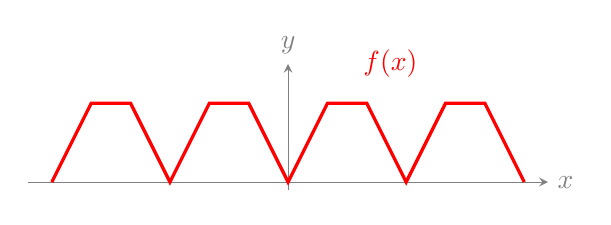
\begin{tikzpicture}[>=stealth]
    \draw[gray,->] (-3.3,0) -- (3.3,0) node[right] {$x$};
    \draw[gray,->] (0,-.1) -- (0,1.5) node[above] {$y$};
    \draw[very thick,red] (-3,0) -- 
    (-2.5,1) -- (-2,1) --
    (-1.5,0) -- (-1,1) -- 
    (-0.5,1) -- (0,0) -- 
    (0.5,1) -- (1,1) -- 
    (1.5,0) -- (2,1) -- 
    (2.5,1) -- (3,0);
    \node[red] at (1.3,1.5) {$f(x)$};
  \end{tikzpicture}
  \caption{Función periódica.}
\end{figure}

Se considera también la frecuencia $f=\frac{1}{T}$, que indica la cantidad de repeticiones de $f(x)$ en determinado intervalo. De aquí también sale $\omega = 2\pi f$, que solo difiere de $f$ en un factor de $2\pi$.

Una propiedad fundamental es que la suma de dos o más funciones periódicas también es periódica. Por ejemplo, dadas $f$ y $g$ periódicas:
$$
\left. \begin{aligned} f(x)=f(x+nT) \\
g(x)=g(x+nT) \end{aligned} \right\} h(x) = af(x) + bg(x) = h(x+nT)
$$
donde $a$ y $b$ son constantes arbitrarias.
\begin{figure}[ht]
  \centering
  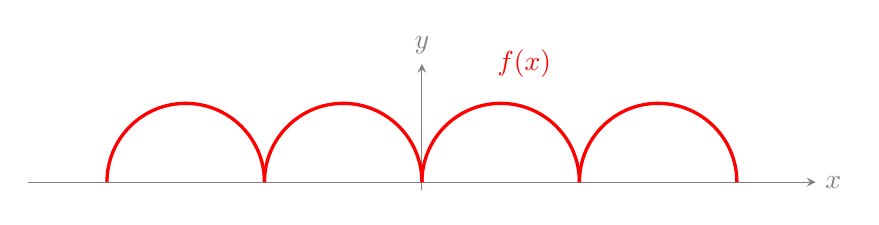
\begin{tikzpicture}[>=stealth]
    \draw[gray,->] (-5,0) -- (5,0) node[right] {$x$};
    \draw[gray,->] (0,-.1) -- (0,1.5) node[above] {$y$};
    \foreach \x in {-4,-2,0,2} {
      \draw[red,very thick] (\x,0) arc (180:0:1);
    }
    \node[red] at (1.3,1.5) {$f(x)$};
  \end{tikzpicture}
  \begin{tikzpicture}[>=stealth]
    \draw[gray,->] (-5,0) -- (5,0) node[right] {$x$};
    \draw[gray,->] (0,-.1) -- (0,1.5) node[above] {$y$};
    \foreach \x in {-3,-1,1,3} {
      \draw[blue,very thick] 
        ($(\x-0.3,0)$) -- ($(\x-0.3,0.3)$) -- ($(\x+0.3,0.3)$) -- ($(\x+0.3,0)$);
    }
    \node[blue] at (1.3,1) {$g(x)$};
  \end{tikzpicture}
  \begin{tikzpicture}[>=stealth]
    \draw[gray,->] (-5,0) -- (5,0) node[right] {$x$};
    \draw[gray,->] (0,-.1) -- (0,1.8) node[above] {$y$};
    \foreach \x in {-4,-2,0,2} {
      \draw[violet!50,very thick] (\x,0) arc (180:0:1);
    }
    \foreach \x in {-3,-1,1,3} {
      \draw[violet!50,very thick,fill=white] 
        ($(\x-0.3,0.93)$) -- ($(\x-0.3,1.3)$) -- ($(\x+0.3,1.3)$) -- ($(\x+0.3,0.93)$);
    }
    \node[violet!50] at (1.3,1.8) {$h(x)$};
  \end{tikzpicture}
  \caption{Suma de funciones periódicas.}
\end{figure}

Lo que posibilita que, sumando funciones trigonométricas se pueda aproximar una función periódica arbitraria.

\section{Serie de Fourier}

La serie de Fourier trigonométrica es una herramienta matemática que permite representar una función \textit{periódica} como una suma infinita de senos y cosenos.

\begin{definition}
Sea $f(x)$ una función real periódica. Su serie de Fourier trigonométrica es
$$
f(x) = a_0 + \sum_{n=1}^{\infty} \big( a_n \cos(nx) + b_n \sin(nx) \big),
$$
\end{definition}

Desarrollando la serie:
\begin{gather*}
  f(x)= a_0 + \color{blue!60}[a_1 \cos(x) + b_1 \sin(x)]\color{black} + \color{red!60}[a_2 \cos(2x) + b_2 \sin(2x)]\color{black} + \cdots\\ 
  \cdots + \color{orange!80}[a_n \cos(nx)+b_n \sin(nx)]\color{black} + \cdots
\end{gather*}
donde todos los términos son periódicos, incluido $a_0$ que es constante, que también cumple con la definición de periodicidad $a_0(x)=a_0(x+nT)$.
Dejando de lado a $a_0$, para cada valor de $n$:
\begin{itemize}
  \item $\color{blue!60}a_1\cos(x)+b_1\sin(x)$ se llama primer armónico, y es el armónico fundamental.
  \item $\color{red!60}a_2\cos(2x)+b_2\sin(2x)$ se llama segundo armónico,
  \item $\color{orange!80}a_n\cos(nx)+b_n\sin(nx)$ se llama $n$-ésimo armónico.
\end{itemize}
donde $a_0$, $a_n$ y $b_n$ son coeficientes a determinar.

\section{Revisión: Conceptos de Algebra Lineal}

Para calcular los coeficientes es útil recordar algunos conceptos.

\subsection{Ortogonalidad}

En \texttt{Algebra Lineal} vimos lo que es ser ortogonal. Digamos dado un conjunto de elementos, el conjunto era ortogonal si y solo si el producto escalar entre todos los elementos es cero:
$$
C=\{a,b,c,\cdots\}
$$
Entonces, $C$ es ortogonal si:
\begin{gather*}
\langle a,b\rangle = \langle a,c\rangle = \cdots =0 \\
\langle b,c\rangle = \langle b,d\rangle = \cdots =0 \\
\qquad \vdots
\end{gather*}

Por ejemplo, digamos que tenemos un conjunto $A=\{f(x),g(x)\}$ de dos funciones. $A$ es un conjunto ortogonal si:
$$
\langle f(x),g(x)\rangle = 0
$$

¿Y cómo era el producto escalar entre funciones? Muy sencillo. El producto escalar entre funciones se define de la siguiente manera:
$$
\langle f,g\rangle = \int_a^b (f\cdot g) \, dx
$$
Entonces, se dice que $f$ es ortogonal a $g$ en el intervalo $[a,b]$ si el resultado de dicha integral definida es cero.

\subsection{Ortonormalidad}

Ser ortonormal, no es más que ser ortogonal y normado al mismo tiempo. ¿Qué era ser normado? Básicamente que la norma sea unitaria (uno). Veamos, si tenemos una función $f$ y queremos ver su norma, entonces, no es necesario recordar cómo se calculaba la norma, ya que, como sabemos el producto escalar, podemos usar la \textit{norma inducida por el producto escalar}. Esto era:
$$
\lVert f \rVert = \sqrt{\langle f,f\rangle} = \sqrt{\int_a^b f^2(x)\,dx}
$$
Entonces, si $f$ es una función ortonormal en el intervalo $[a,b]$:
$$
\lVert f \rVert = \sqrt{\int_a^b f^2(x)\,dx} =1
$$
Y si no es normal se puede dividir por su norma para que sea normal.

Veamos un ejemplo otra vez para clarificar. Continuemos con el conjunto $A=\{f(x),g(x)\}$. Este conjunto será ortonormal en $[a,b]$ si:
\begin{gather*}
\langle f(x),g(x)\rangle = \int_a^b (f(x)\cdot g(x))\, dx = 0\\[7pt]
\lVert f(x) \rVert = \sqrt{\int_a^b f(x)^2\,dx} = 1\\[7pt]
\lVert g(x) \rVert = \sqrt{\int_a^b g(x)^2\,dx} = 1
\end{gather*}
Es decir, todos los elementos del conjunto (la familia de vectores) es ortogonal y cada elemento del conjunto, es normal. En este caso decimos que $A$ es ortonormal.

¿Y para qué es necesario recordar todo eso? Porque un ejemplo de conjunto ortogonal son las funciones trigonométricas en el intervalo $[-\pi,\pi]$.

Digamos, por ejemplo que definimos la siguiente familia de senos:
$$
S = \{\sin(nx) ~|~ n\in\mathbb{Z} \}
$$
Entonces nos preguntamos ¿Es esta familia ortogonal? Para responder nos damos dos números enteros distintos: $a,b \in \mathbb{Z}$ con $a\neq b$. Entonces $S$ es ortogonal si $\langle \sin(ax),\sin(bx)\rangle = 0 \quad \forall a,b \in \mathbb{Z}$ 
$$
\int_{-\pi}^\pi \sin(ax) \sin(bx) \, dx
$$
Para resolver la integral es útil usar la siguiente relación:
$$
\sin(ax)\sin(bx) = \frac{1}{2}[\cos((a-b)x) - \cos((a+b)x)]
$$
Aplicando la propiedad trigonométrica y distribuyendo la integral:
\begin{equation}
\frac{1}{2}\left[ \int_{-\pi}^\pi \cos((a-b)x)\,dx - \int_{-\pi}^\pi \cos((a+b)x)\,dx \right]
\label{eq:relacion_integral_trigonometrica_fourier}
\end{equation}
Esta integral si sabemos resolverla, son integrales de cosenos:
$$
\int_{-\pi}^\pi \cos((a-b)x)\,dx = \left. \frac{\sin((a-b)x)}{a-b} \right\rvert_{-\pi}^\pi = \frac{\sin((a-b)\pi)- \sin((a-b)(-\pi))}{a-b}
$$
Como $a-b\in\mathbb{Z}$, llamamos $k = a-b$ y como $\sin(-x)=-\sin(x)$ la expresión queda:
$$
\int_{-\pi}^\pi \cos((a-b)x)\,dx =\frac{\sin((a-b)\pi)+ \sin((a-b)(\pi))}{a-b}
$$
Como $\sin(k\pi)=0$ con $k\in\mathbb{Z}$, resulta:
$$
\int_{-\pi}^\pi \cos((a-b)x)\,dx = 0
$$
Entonces reemplazamos este resultado en \eqref{eq:relacion_integral_trigonometrica_fourier} queda:
$$
\frac{1}{2}\left[ 0 - \int_{-\pi}^\pi \cos((a+b)x)\,dx \right]
$$
La segunda integral también da cero, se puede demostrar de la misma manera que se hizo con la primera. Esto resulta entonces en:
\begin{gather*}
\int_{-\pi}^\pi \sin(ax) \sin(bx) \, dx = 0 \\[7pt]
\therefore ~ S \text{ es ortogonal }\forall a,b \in \mathbb{Z}
\end{gather*}
Esto concluye que el conjunto $S$ de todas las funciones seno de la forma $\sin(nx)$ con $n\in\mathbb{Z}$ es ortogonal. Ahora podríamos preguntarnos ¿Es ortonormal? Usando la norma inducida por el producto tenemos:
$$
\lVert\sin(ax)\rVert = \sqrt{\int_{-\pi}^\pi \sin^2(ax)\, dx}
$$
Observando la integral, para resolverla necesitamos operar sobre el seno. Usando la misma propiedad de recién (solo que esta vez $a=b$) queda:
\begin{align*}
\int_{-\pi}^\pi \sin^2(ax)\, dx &= \int_{-\pi}^\pi \frac{1-\cos(2ax)}{2}dx \\[7pt]
								&= \int_{-\pi}^\pi \frac{1}{2}dx-\int_{-\pi}^\pi \frac{\cos(2ax)}{2}dx \\[7pt]
								&=\left. \frac{x}{2}\right\lvert_{-\pi}^\pi - \left. \frac{\sin(2ax)}{4a} \right\lvert_{-\pi}^\pi \\[7pt]
								&= \frac{\pi}{2} + \frac{\pi}{2} - 0 = \boxed{\pi}
\end{align*}
Entonces:
$$
\lVert\sin(ax)\rVert = \sqrt{\int_{-\pi}^\pi \sin^2(ax)\, dx} = \sqrt{\pi}
$$
Esto significa que no es un conjunto ortonormal. Sin embargo podemos convertirlo en uno dividiendo cada una de las funciones del conjunto por la norma que obtuvimos:
$$
S'= \left\{\frac{\sin(nx)}{\sqrt{\pi}} ~ \Bigg\lvert ~ n\in\mathbb{Z}\right\}
$$
Ahora si, $S'$ es un conjunto ortonormal. Esto lo usaremos para deducir los coeficientes: $a_0,a_n$ y $b_n$.

\section{Cálculo de los coeficientes de Fourier}

El cálculo de los coeficientes $a_0,a_n$ y $b_n$ de la serie trigonométrica de Fourier requieren los conceptos de conjuntos ortonormales que ya vimos. Vamos a partir de integrar en el intervalo $[-\pi,\pi]$ para encontrar el primer coeficiente: $a_0$
\begin{gather*}
f(x) = a_0 + \sum_{n=1}^\infty (a_n \cos(nx) + b_n\sin(nx)) \\[10pt]
\int_{-\pi}^\pi f(x)\, dx = \int_{-\pi}^\pi a_0 \, dx + \int_{-\pi}^\pi \sum_{n=1}^\infty(a_n \cos(nx) + b_n\sin(nx)) \, dx
\end{gather*}
Para poder integrar sobre la serie infinita, necesitamos asegurar convergencia uniforme de la serie. Esto puede demostrarse y asegurarse para funciones trigonométricas que forman un sistema ortogonal en el espacio $L^2([-\pi,\pi])$. Esto se fundamenta usando espacios de Hilbert, y no se demostrará.

\subsection[Primer coeficiente]{Coeficiente $a_0$}

Partiendo entonces de 
\begin{align*}
\int_{-\pi}^\pi f(x)\, dx &= \int_{-\pi}^\pi a_0 \, dx + \int_{-\pi}^\pi \sum_{n=1}^\infty(a_n \cos(nx) + b_n\sin(nx)) \, dx \\[10pt]
						  &= a_0(2\pi) + \sum_{n=1}^\infty \left[ a_n \int_{-\pi}^\pi\cos(nx)\,dx + b_n \int_{-\pi}^\pi \sin(nx) \, dx \right] \\[10pt]
						  &= a_0(2\pi) + \sum_{n=1}^\infty \left[ a_n \cancel{\frac{\sin(nx)}{n}} \Big\rvert_{-\pi}^\pi - b_n \frac{\cos(nx)}{n}\Big\rvert_{-\pi}^\pi \right] \\[10pt]
						  &= 2\pi a_0 + \sum_{n=1}^\infty -b_n \left( \frac{\cos(n\pi) - \cos(n(-\pi))}{n} \right)
\end{align*}
Y como $\cos(n\pi)=\cos(n(-\pi))$
\begin{align*}
\int_{-\pi}^\pi f(x)\, dx &= 2\pi a_0 + \sum_{n=1}^\infty -b_n \cancel{\frac{\cos(n\pi)-\cos(n\pi)}{n}} \\[10pt]
\int_{-\pi}^\pi f(x)\, dx &= 2\pi a_0 
\end{align*}
Como buscamos $a_0$, despejamos:
$$
\boxed{a_0 = \frac{1}{2\pi}\int_{-\pi}^\pi f(x)\,dx}
$$

\subsection[Segundo coeficiente]{Coeficiente $a_n$}

Partimos de la forma de la serie de Fourier en $[-\pi,\pi]$:
$$
f(x) = a_0 + \sum_{n=1}^\infty \big(a_n \cos(nx) + b_n \sin(nx)\big).
$$
La estrategia para encontrar $a_n$ es parecida a la que tomamos para encontrar $a_0$. La única diferencia es que esta vez vamos a multiplicar ambos lados por $\cos(mx)$ donde $m\in\mathbb{Z}$ es un entero \textbf{fijo} y luego, como hicimos anteriormente, integrar de $-\pi$ a $\pi$. Esto se hace porque los senos y cosenos tienen propiedades de ortogonalidad muy simples en ese intervalo. Aquí lo importante es que eventualmente, $n=m$ cuando se tomen distintos valores de $n$ en la serie infinita. 

Para enteros $m,n\ge1$ vale la relación
$$
\int_{-\pi}^{\pi}\cos(mx)\cos(nx)\,dx =
\begin{cases}
0, & m\neq n,\\[4pt]
\pi, & m=n,
\end{cases}
$$
y también,
$$
\int_{-\pi}^{\pi}\cos(mx)\sin(nx)\,dx = 0,
\qquad
\int_{-\pi}^{\pi}\cos(mx)\,dx = 0.
$$
Estas tres identidades las usaremos para despejar $a_n$ y quitar la suma infinita. Con esto en mente, multiplicamos la serie por $\cos(mx)$ e integramos:
\begin{align*}
\int_{-\pi}^\pi f(x)\cos(mx)\,dx
=&~ a_0 \int_{-\pi}^\pi \cos(mx)\,dx + \\
&+ \sum_{n=1}^\infty a_n \int_{-\pi}^\pi \cos(nx)\cos(mx)\,dx + \\
&+ \sum_{n=1}^\infty b_n \int_{-\pi}^\pi \sin(nx)\cos(mx)\,dx
\end{align*}
Multiplicar la serie por $\cos(mx)$ y luego integrar corresponde a calcular el producto escalar $\langle f,\cos(mx)\rangle$. Dado que las funciones $\{\cos(nx),\sin(nx)\}_{n\ge1}$ son ortogonales en el intervalo $[-\pi,\pi]$, todos los términos cruzados desaparecen salvo el de $n=m$. Eso ``aisla'' el coeficiente $a_m$. Para conseguir esto, aplicamos las identidades mencionadas:
\begin{itemize}
  \item El término con $a_0$ desaparece porque $\int_{-\pi}^\pi \cos(mx)\,dx = 0$.
  \item Toda la suma de los $b_n$ desaparece porque $\sin$ y $\cos$ son ortogonales.
  \item En la suma de los $a_n$, todos los términos se anulan salvo el de $n=m$.
\end{itemize}
Con esto, en la suma sólo sobrevive el término con $n=m$:
\begin{equation}
\int_{-\pi}^\pi f(x)\cos(mx)\,dx = a_m \int_{-\pi}^\pi \cos^2(mx)\,dx.
\label{eq:termino_an}
\end{equation}
Ahora, solo queda evaluar la integral. Sabemos que
$$
\cos^2(mx) = \frac{1+\cos(2mx)}{2},
$$
así que
\begin{align*}
  \int_{-\pi}^\pi \cos^2(mx)\,dx &= \int_{-\pi}^\pi \frac{1+\cos(2mx)}{2}\,dx \\ 
                                 &= \frac{1}{2}\int_{-\pi}^\pi 1\,dx + \frac{1}{2}\int_{-\pi}^\pi \cos(2mx)\,dx.
\end{align*}
El segundo término es cero por integrarse sobre un múltiplo del período. El primero vale $\pi$. Por lo tanto:
$$
\int_{-\pi}^\pi \cos^2(mx)\,dx = \pi.
$$
Entonces reemplazando este resultado en \eqref{eq:termino_an}:
$$
\int_{-\pi}^\pi f(x)\cos(mx)\,dx = a_m \pi.
$$
Donde obtenemos 
$$
a_m = \frac{1}{\pi}\int_{-\pi}^\pi f(x)\cos(mx)\,dx
$$
Y, como $m\in\mathbb{Z}$ es fijo, pero cualquier entero, nos permite encontrar un término genérico, siendo así posible encontrar la ley de formación  
$$
\boxed{a_n = \frac{1}{\pi}\int_{-\pi}^\pi f(x)\cos(nx)\,dx.}
$$
Observe el precioso detalle: esta conexión de la serie de Fourier y el álgebra lineal (familia de vectores más en concreto), nos permite entender a la serie de Fourier como una familia libre de funciones periódicas seno y coseno que generan un espacio vectorial de funciones periódicas de periodo $2\pi$ en este caso. De esta manera, se puede ver a una función $f$ representada por la serie de Fourier como una combinación lineal infinita de los infinitos vectores de la base (dados por la propia serie). Esto es lo que nos permite representar cualquier función periódica $f$ que forme parte del espacio vectorial generado por la base.

\subsection[Último coeficiente]{Coeficiente $b_n$}

Aquí ya podemos intuir cómo se obtendrá la forma de cálculo de este coeficiente. Aquí, a diferencia del coeficiente $a_n$ donde multiplicamos por $\cos(mx)$ para eliminar $b_n$, ahora vamos a multiplicar por $\sin(mx)$ para eliminar $a_n$.

Entonces, partimos de la serie de Fourier:
$$
f(x)=a_0 + \sum_{n=1}^\infty a_n \cos(nx) + b_n \sin(nx)
$$
Siguiendo el razonamiento que hicimos en $a_n$, multiplicamos miembro a miembro por $\sin(mx)$ y luego integramos en el intervalo $[-\pi,\pi]$.
\begin{align}
\int_{-\pi}^\pi f(x)\cdot\sin(mx)\, dx  =&~ a_0 \int_{-\pi}^\pi \sin(mx) \,dx +\notag \\
										&+ \sum_{n=1}^\infty a_n \int_{-\pi}^\pi \cos(nx)\sin(mx) \,dx +\notag \\ 
                    &+ \sum_{n=1}^\infty b_n \int_{-\pi}^\pi \sin(nx)\sin(mx) \,dx\label{eq:serie_bn}
\end{align}
Sabemos que:
\begin{gather}
  \int_{-\pi}^\pi \sin(mx) \,dx=0 \quad \forall m\in\mathbb{Z} \label{eq:bn_1}\\
  \int_{-\pi}^\pi \cos(nx)\sin(mx) \,dx = 0 \quad \forall n,m \in \mathbb{Z}\label{eq:bn_2} \\
  \int_{-\pi}^\pi \sin(nx)\sin(mx) \,dx = \begin{cases}0 & n\neq m \\ \pi & n=m\end{cases}\label{eq:bn_3}
\end{gather}
La justificación de esto es análogo a las justificaciones de $a_n$, es decir, para \eqref{eq:bn_2} tenemos que es 0 ya que $\sin(mx)$ y $\cos(nx)$ son ortogonales. Y para \eqref{eq:bn_3} tenemos que $\sin(nx)$ es ortogonal a $\sin(mx)$ siempre que $n\neq m$. En el caso especial donde $n=m$ estamos calculando $\lVert \sin(mx)\rVert^2=\pi$.

Reemplazando los resultados \eqref{eq:bn_1}, \eqref{eq:bn_2} y \eqref{eq:bn_3} en la serie ecuación \eqref{eq:serie_bn}:
$$
\int_{-\pi}^\pi f(x)\cdot\sin(mx) \,dx = 0 + 0 + b_m \pi
$$
De este modo solo despejamos $b_m$ y, como $m\in\mathbb{Z}$ es genérico, obtenemos la ley de formación de $b_n$:
$$
\boxed{b_n = \frac{1}{\pi}\int_{-\pi}^\pi f(x)\cdot\sin(nx) \,dx}
$$

\section{Fourier para funciones de periodo arbitrario}

Pueden haber funciones $f(t)$ con periodo arbitrario $T$ tal que $T\neq 2\pi$. La idea es plantear un cambio de variable lineal que ajusta la escala del periodo. En el caso estándar de Fourier trabajamos en $[-\pi, \pi]$, donde el periodo es $2\pi$. Pero si una función $f(t)$ tiene periodo $T$, lo natural es trabajar en un intervalo de longitud $T$, por ejemplo $[-T/2,T/2]$.

Entonces necesitamos un cambio de variable que convierta:
$$
[-T/2, \, T/2] \quad \longrightarrow \quad [-\pi, \, \pi].
$$
Ese cambio de variable es simplemente una homotecia:
$$
x = \frac{2\pi}{T} t.
$$
Este ``estiramiento'' hace que un ciclo de longitud $T$ en $t$ se convierta en un ciclo de longitud $2\pi$ en $x$. Evidentemente, este cambio de variable debemos aplicarlo a la integral, para ello se necesita expresar $dt$ en términos de $dx$ (o viceversa). De $x = \frac{2\pi}{T}t$, se deduce:
$$
dx = \frac{2\pi}{T}\,dt \quad \Longleftrightarrow \quad dt = \frac{T}{2\pi}\,dx.
$$
Esto es simplemente la regla de diferenciación. Así, la serie de Fourier para período arbitrario $T$ resulta
$$
f(t)=a_0 + \sum_{n=1}^\infty a_n \cos\left(\frac{2n\pi}{T}t\right) + b_n \sin\left(\frac{2n\pi}{T}t\right)
$$
donde, los coeficientes se calculan de la siguiente manera
\begin{align*}
  a_0 &= \frac{1}{T}\int_{-T/2}^{T/2} f(t) \,dt \\ 
  a_n &= \frac{2}{T}\int_{-T/2}^{T/2} f(t)\cos\left(\frac{2n\pi}{T}t\right) \,dt \\
  b_n &= \frac{2}{T}\int_{-T/2}^{T/2} f(t)\sin\left(\frac{2n\pi}{T}t\right) \,dt
\end{align*}

\subsection{Sobre el tipo de paridad}

Dependiendo de la paridad de $f$ se tendrán distintos términos en la serie de Fourier. Una $f(t)$ puede:
\begin{enumerate}
  \item No presentar simetría (tendrá $a_0$, $a_n$ y $b_n$)
  \item Presentar simetría par
  \item Presentar simetría impar
\end{enumerate}
Y dependiendo de su paridad, se aplicarán determinadas propiedades.

\begin{property}(Simetría par)
Si $g(t)=-g(t)$ es par; y si $g$ además es periódica con periodo $T$, se cumple:
$$
\int_{-T/2}^{T/2} g(t)\,dt = 2 \int_{0}^{T/2}g(t)\, dt
$$
\label{prop:simetria_par}
\end{property}
\begin{property}(Simetría impar)
Si $h(t)=-h(-t)$ es impar; y además $h$ es periódica de periodo $T$, se cumple que:
$$
\int_{-T/2}^{T/2} h(t)\,dt = 0
$$
\label{prop:simetria_impar}
\end{property}

\subsection{Desarrollo de la serie: par e impar}

Teniendo en cuenta lo anterior y la siguiente propiedad: 
\begin{property}(Paridad de operaciones)
  Si se tienen dos funciones $f$ y $g$ multiplicadas, se cumple
  \begin{itemize}
    \item $f$ par $\times$ $g$ par $\Rightarrow ~ f\cdot g$ es par.
    \item $f$ impar $\times$ $g$ impar $\Rightarrow ~ f\cdot g$ es par.
    \item $f$ par $\times$ $g$ impar $\Rightarrow ~ f\cdot g$ es impar.
  \end{itemize}
  \label{prop:paridad_de_op}
\end{property}

\paragraph{Desarrollo par}

Si se desea representar una $f(t)$ de periodo arbitrario $T$ en serie de Fourier y $f$ es par, entonces su serie de Fourier tendrá la forma
$$
f(t)=a_0 + \sum_{n=1}^\infty a_n \cos\left(\frac{2n\pi}{T}t\right)
$$
tras aplicar las propiedades \ref{prop:simetria_par} y \ref{prop:paridad_de_op}.
 
\paragraph{Desarrollo Impar}

Si se desea representar una $f(t)$ de periodo arbitrario $T$ en serie de Fourier y $f$ es impar, entonces su serie de Fourier tendrá la forma
$$
f(t)=a_0 + \sum_{n=1}^\infty b_n \sin\left(\frac{2n\pi}{T}t\right)
$$
tras aplicar las propiedades \ref{prop:simetria_impar} y \ref{prop:paridad_de_op}.

\section{Desarrollo de medio rango}

Hay un caso excepcional en el cual una función no periódica puede ser representada en Serie de Fourier, siempre y cuando la función esté definida en un intervalo arbitrario y no exista fuera de ese intervalo. Es decir, una función que esté definida en el intervalo $[0,L]$. 
\begin{figure}[ht]
  \centering
  \begin{tikzpicture}[>=stealth]
    \draw[gray,->] (-0.1,0) -- (3.5,0) node[right] {$t$};
    \draw[gray,->] (0,-0.1) -- (0,2) node[above] {$f(t)$};
    \draw[dotted,gray] (3,0) node[below] {$\ell$} -- (3,1.5);
    \draw[very thick, red] (0,0.5) -- (1,0.5) to [out=0,in=230] (3,1.5);
  \end{tikzpicture}
  \caption{Función definida en el intervalo $[0,\ell]$.}
  \label{fig:periodo_ele}
\end{figure}
Supongamos que existe una cierta función del tiempo $f(t)$ definida en el intervalo $[0,\ell]$, siendo el campo de existencia de $f:0\leqslant t \leqslant \ell$, gráficamente, podría ser una función como la de la figura \ref{fig:periodo_ele}.

\subsection{Extensión par}

Consideramos la posibilidad de que exista una cierta función periódica par $g(t)$, tal que, en $0\leqslant t \leqslant \ell$ resulte ser idéntica a $f$ (ver figura \ref{fig:extension_par}).

Como $g$ es periódica par, si tiene desarrollo en serie de Fourier, cuya expresión sera:
\begin{equation}
  g(t)=a_0 + \sum_{n=1}^\infty a_n \cos\left(\frac{2n\pi}{T}t\right)
  \label{eq:extension_par_de_g}
\end{equation}
\begin{figure}[ht]
  \centering
  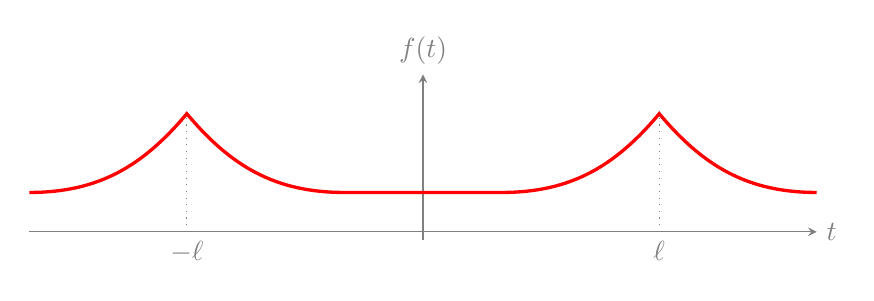
\begin{tikzpicture}[>=stealth]
    \draw[gray,->] (-5,0) -- (5,0) node[right] {$t$};
    \draw[gray,->] (0,-0.1) -- (0,2) node[above] {$f(t)$};
    \draw[dotted,gray] (3,0) node[below] {$\ell$} -- (3,1.5);
    \draw[dotted,gray] (-3,0) node[below] {$-\ell$} -- (-3,1.5);
    \draw[very thick, red] (-5,0.5) to [out=0,in=230] (-3,1.5)
    to [out=310,in=180] (-1,0.5) -- (1,0.5) to [out=0,in=230] (3,1.5)
    to [out=310,in=180] (5,0.5);
  \end{tikzpicture}
  \caption{Extensión periódica par de la función.}
  \label{fig:extension_par}
\end{figure}
Con $T=2\ell$. Por ser $g$ par, $b_n=0$. Entonces, podemos reescribir \eqref{eq:extension_par_de_g} reemplazando $T=2\ell$
$$
g(t) = a_0 + \sum_{n=1}^\infty a_n \cos\left(\frac{n\pi}{\ell}t\right)
$$
Si ahora calculamos los coeficientes para $g$:
\begin{align*}
  a_0=\frac{2}{T}\int_0^{T/2}g(t)\,dt &\longrightarrow a_0=\frac{1}{\ell}\int_0^\ell g(t)\,dt \\
  a_n=\frac{4}{T}\int_0^{T/2} g(t)\cos\left(\frac{2n\pi}{T}t\right) \,dt &\longrightarrow a_n = \frac{2}{\ell}\int_0^{\ell} g(t) \cos\left(\frac{n\pi}{\ell}t\right)\,dt
\end{align*}

Observando los coeficientes $a_0$ y $a_n$, vemos que ambos surgen de integrales con extremos $t=0$ y $t=\ell$. Pero en $0\leqslant t\leqslant \ell$ $f(t)$ y $g(t)$ son idénticas (condición del problema), por lo que son intercambiables dentro de la integral con los mismos extremos. El resultado de las integrales será el mismo utilizando $f$ o $g$, entonces redefinimos $a_0$ y $a_n$:
\begin{align*}
  A_0 &= \frac{1}{\ell} \int_0^\ell f(t)\,dt \\
  A_n &= \frac{2}{\ell} \int_0^\ell f(t)\cos\left(\frac{n\pi}{\ell}t\right)\,dt
\end{align*}

Así podemos expresar a $f(t)$ en serie de Fourier, pese a no ser periódica. De este modo, la extensión par de $f$ es:
$$
f(t)=A_0+\sum_{n=1}^\infty A_n \cos\left(\frac{n\pi}{\ell}t\right)
$$

\subsection{Extensión impar}

De la misma forma que en la extensión par, suponemos que existe una función $h(t)$ tal que es igual a la función $f(t)$ en el intervalo $[0,\ell]$, donde $h(t)$ es función periódica impar (ver figura \ref{fig:extension_impar}).
\begin{figure}[ht]
  \centering
  \begin{tikzpicture}[>=stealth]
    \draw[gray,->] (-5,0) -- (5,0) node[right] {$t$};
    \draw[gray,->] (0,-2) -- (0,2) node[above] {$f(t)$};
    \draw[dotted,gray] (3,0) node[below] {$\ell$} -- (3,1.5);
    \draw[dotted,gray] (-3,0) node[above] {$-\ell$} -- (-3,-1.5);
    \draw[very thick, red] (-5,-0.5) to [out=0,in=-230] (-3,-1.5)
    to [out=-310,in=-180] (-1,-0.5) -- (0,-0.5);
    \draw[very thick, red] (0,0.5) -- (1,0.5) to [out=0,in=230] (3,1.5)
    to [out=310,in=180] (5,0.5);
  \end{tikzpicture}
  \caption{Extensión periódica impar de la función.}
  \label{fig:extension_impar}
\end{figure}
Cuyo desarrollo en serie de Fourier es:
$$
h(t)=\sum_{n=1}^\infty b_n \sin\left(\frac{2n\pi}{T}t\right)
$$
Siguiendo la misma lógica que para la extensión par $T=2\ell$, entonces:
$$
h(t)=\sum_{n=1}^\infty b_n \sin\left(\frac{n\pi}{\ell}t\right)
$$
Donde 
$$
b_n = \frac{2}{\ell} \int_0^\ell h(t)\sin\left(\frac{n\pi}{\ell}t\right)\,dt
$$
Y como $h(t)=f(t)$ en el intervalo $[0,\ell]$, aplicamos la sustitución:
$$
B_n = \frac{2}{\ell}\int_0^\ell f(t)\sin\left(\frac{n\pi}{\ell}t\right)\,dt
$$
Y la extensión impar de $f$ es:
$$
f(t)=\sum_{n=1}^\infty B_n\sin\left(\frac{n\pi}{\ell}t\right)
$$

\section[Expresión exponencial de la Serie de Fourier]{Expresión exponencial de la Serie de \\ Fourier}

A partir de la trigonométrica de Fourier, se puede enunciar la serie en su forma exponencial usando ecuaciones de Euler\footnote{Leonhard Paul Euler: matemático y físico suizo.}, que relacionan a las funciones trigonométricas y exponenciales.

Dada 
$$
f(x)=a_0+\sum_{n=1}^\infty\left[a_n\cos(nx)+b_n\sin(nx)\right]
$$
y recordando:
\begin{gather}
  \cos(nx)=\frac{e^{jnx}+e^{-jnx}}{2} \quad \text{y} \quad \sin(nx)=\frac{e^{jnx}-e^{-jnx}}{2j} \\ 
  e^{jnx}=\cos(nx)+j\sin(nx) \quad \text{y}\quad e^{-jnx}=\cos(nx)-j\sin(nx) \notag
  \label{eq:relaciones_de_euler}
\end{gather}
Si reemplazamos con las relaciones \eqref{eq:relaciones_de_euler} en la expresión trigonométrica de Fourier, resulta:
\begin{align*}
f(x)&=a_0+ \sum_{n=1}^\infty a_n \frac{e^{jnx}+e^{-jnx}}{2} + b_n \frac{e^{jnx}-e^{-jnx}}{2j}\\[8pt]
&=a_0 + \sum_{n=1}^\infty a_n\frac{e^{jnx}}{2} + a_n\frac{e^{-jnx}}{2} + b_n\frac{e^{jnx}}{2j} - b_n \frac{e^{-jnx}}{2j} \\[8pt]
&=a_0 + \sum_{n=1}^\infty e^{jnx}\left(\frac{a_n}{2}+\frac{b_n}{2j}\right) + e^{-jnx}\left(\frac{a_n}{2}-\frac{b_n}{2j}\right)
\end{align*}
Como $j^{-1}=-j$
$$
f(x)= a_0 + \sum_{n=1}^\infty \left(\frac{a_n}{2}-j\frac{b_n}{2}\right)e^{jnx} + \left(\frac{a_n}{2}+j\frac{b_n}{2}\right)e^{-jnx}
$$
Entonces, ahora podemos realizar la siguiente sustitución:
\begin{itemize}
  \item $A_0=a_0$
  \item $A_n=\frac{a_n}{2}-j\frac{b_n}{2}=\frac{1}{2}(a_n-jb_n)$
  \item $B_n=\frac{a_n}{2}+j\frac{b_n}{2}=\frac{1}{2}(a_n+jb_n)$
\end{itemize}
Quedando:
$$
\boxed{f(x)=A_0 + \sum_{n=1}^\infty A_n e^{jnx} + B_n e^{-jnx}}
$$
Ahora debemos encontrar la forma de calculo de $A_n$ y $B_n$:
\begin{gather*}
A_n =\frac{1}{2}(a_n-jb_n) = \\ 
=\frac{1}{2}\left( \frac{2}{T}\int_{-T/2}^{T/2}f(x)\cos\left(\frac{2n\pi}{T}t\right)\,dt ~~ - ~~ j\frac{2}{T}\int_{-T/2}^T f(x)\sin\left(\frac{2n\pi}{T}t\right)\,dt \right)\\
= \frac{1}{T}\int_{-T/2}^{T/2}f(x)\cdot \left[\cos\left(\frac{2n\pi}{T}t\right) - j\sin\left(\frac{2n\pi}{T}t\right)\right]\,dt
\end{gather*}
Como sabemos que $e^{-jx}=\cos(x)-j\sin(x)$:
$$
\boxed{
A_n = \frac{1}{T}\int_{-T/2}^{T/2}f(x)\cdot e^{-j\frac{2n\pi}{T}t}\,dt
}
$$
Y siguiendo la misma lógica para $B_n$, y usando $e^{jx}=\cos(x)+j\sin(x)$ como relación:
$$
\boxed{
B_n = \frac{1}{T}\int_{-T/2}^{T/2}f(x)\cdot e^{j\frac{2n\pi}{T}t}\,dt
}
$$
Nótese que no hemos deducido $A_0$, ya que su forma de cálculo es la misma.

\section{Serie compleja de Fourier}

Observando $A_n$ y $B_n$ del desarrollo anterior, vemos que solo difieren en el signo exponencial. Es decir, podríamos reescribir la serie como:
$$
f(x)=A_0 + \sum_{n=1}^\infty A_n e^{jnx} + A_{(-n)}e^{-jnx}
$$
Observando la variación de $n$, se puede considerar que varia desde $-\infty$ a $\infty$, pasando por cero con $A_0$. Donde $n$, una variable discreta, varía por saltos y no en forma continua $~\therefore ~$ con su versión negativa $(-n)$ se cubre la variación de $(-1)$ a $(-\infty)$ y $(+n)$ de $(1)$ a $(+\infty)$ con valor central $A_0$ para $n=0$, quedando entonces:
$$
\boxed{f(x)=\sum_{-\infty}^\infty C_n e^{jnx}}
\quad  \text{(Fourier compleja)}
$$
Donde $C_n$ viene dado por:
$$
C_n=\frac{1}{T}\int_{-T/2}^{T/2}f(x)\cdot e^{-j\frac{2n\pi}{T}t}\,dt
$$
para $-\infty<n<\infty$.

Es importante entender que si queremos tomar una aproximación, de 20 términos por ejemplo, (como en la serie trigonométrica), no podemos hacer una sumatoria hasta $S_20$ tomando la suma:
$$
\sum_{n=1}^{20} C_n e^{jnx}
$$
Lo correcto es tomar la suma sabiendo que el intervalo ahora está partido en el eje de los enteros:
$$
\sum_{-20}^{20} C_n e^{jnx}
$$

Para finalizar la idea, veamos un ejemplo.

\section{Ejemplo de aplicación: Onda Cuadrada}

Analicemos el desarrollo en serie de Fourier para la función onda cuadrada definida por:
$$
f(t) = \begin{cases}
\phantom{-}2 & -1 < t < 0 \\
-2 & \phantom{-}0 < t < 1
\end{cases}
$$
con periodo $T=2$.

\subsection{Análisis de simetría}

Antes de calcular integrales, es fundamental inspeccionar la gráfica de la función para aprovechar las propiedades de paridad.

\begin{figure}[ht]
  \centering
  \begin{tikzpicture}[>=stealth]
    \draw[gray,->] (-3.5,0) -- (3.5,0) node[right] {$t$};
    \draw[gray,->] (0,-2.5) -- (0,2.5) node[above] {$f(t)$};
    
    % Ejes y etiquetas
    \foreach \x in {-3,-2,-1,1,2,3} \draw[gray] (\x,0.1) -- (\x,-0.1) node[below] {\footnotesize \x};
    \draw[gray] (0.1,2) -- (-0.1,2) node[left] {\footnotesize 2};
    \draw[gray] (0.1,-2) -- (-0.1,-2) node[left] {\footnotesize -2};

    % Función (Onda cuadrada invertida)
    \draw[red, very thick] (-3,2) -- (-2,2); % -3 a -2
    \draw[red, very thick] (-2,-2) -- (-1,-2); % -2 a -1
    \draw[red, very thick] (-1,2) -- (0,2); % -1 a 0
    \draw[red, very thick] (0,-2) -- (1,-2); % 0 a 1
    \draw[red, very thick] (1,2) -- (2,2); % 1 a 2
    \draw[red, very thick] (2,-2) -- (3,-2); % 2 a 3
    
    % Líneas discontinuas para los saltos (opcional, para guiar la vista)
    \draw[red, dashed] (0,-2) -- (0,2);
    \draw[red, dashed] (-1,-2) -- (-1,2);
    \draw[red, dashed] (1,-2) -- (1,2);
    \draw[red, dashed] (2,-2) -- (2,2);
    \draw[red, dashed] (-2,-2) -- (-2,2);
    
  \end{tikzpicture}
  \caption{Función onda cuadrada con $T=2$.}
  \label{fig:onda_cuadrada_ejemplo}
\end{figure}

Observando la figura \ref{fig:onda_cuadrada_ejemplo}, notamos que la función es simétrica respecto al origen, es decir, cumple que $f(t) = -f(-t)$.
\begin{itemize}
    \item Como $f$ es \textbf{impar}, sabemos por la Propiedad \ref{prop:simetria_impar} que todos los coeficientes cosenos son nulos: $a_0 = 0$ y $a_n = 0$.
    \item La serie estará compuesta únicamente por términos senos ($b_n$).
\end{itemize}

\subsection{Cálculo de coeficientes}

Para una función impar con periodo $T=2$ (donde la frecuencia fundamental es $\omega = \frac{2\pi}{T} = \pi$), el coeficiente $b_n$ se simplifica a:
$$
b_n = \frac{4}{T} \int_{0}^{T/2} f(t) \sin\left(\frac{2n\pi}{T}t\right) \,dt
$$
Sustituyendo $T=2$ y el valor de la función en el intervalo positivo ($f(t)=-2$ para $0<t<1$):
\begin{align*}
b_n &= \frac{4}{2} \int_{0}^{1} (-2) \sin(n\pi t) \,dt \\[5pt]
    &= -4 \int_{0}^{1} \sin(n\pi t) \,dt \\[5pt]
    &= -4 \left[ -\frac{\cos(n\pi t)}{n\pi} \right]_0^1 \\[5pt]
    &= \frac{4}{n\pi} \Big[ \cos(n\pi) - \cos(0) \Big]
\end{align*}
Sabemos que $\cos(0)=1$ y $\cos(n\pi)=(-1)^n$. Por tanto:
$$
\boxed{b_n = \frac{4}{n\pi} \left[ (-1)^n - 1 \right]}
$$

Analicemos el comportamiento de este coeficiente según si $n$ es par o impar:
\begin{itemize}
    \item Si $n$ es \textbf{par} ($n=2k$): $(-1)^{2k} - 1 = 1 - 1 = 0$.
    \item Si $n$ es \textbf{impar} ($n=2k+1$): $(-1)^{2k+1} - 1 = -1 - 1 = -2$.
\end{itemize}

Sustituyendo para los impares:
$$
b_n = \frac{4}{n\pi}(-2) = -\frac{8}{n\pi} \quad \text{para } n=1, 3, 5, \dots
$$

\subsection{Construcción de la Serie}

La serie de Fourier queda expresada como:
$$
f(t) = \sum_{n=1, \text{impar}}^\infty \left( -\frac{8}{n\pi} \right) \sin(n\pi t)
$$
Desarrollando los primeros términos para visualizar la aproximación:
$$
f(t) = -\frac{8}{\pi} \sin(\pi t) - \frac{8}{3\pi} \sin(3\pi t) - \frac{8}{5\pi} \sin(5\pi t) - \dots
$$
O usando notación de sumatoria sobre enteros $k$:
$$
f(t) = -\frac{8}{\pi} \sum_{k=0}^{\infty} \frac{1}{2k+1} \sin\big((2k+1)\pi t\big)
$$

\paragraph{Nota sobre convergencia (Fenómeno de Gibbs):}
Como observamos en la figura \ref{fig:fenomeno_gibbs}, aunque la serie converge a la función, en los puntos de discontinuidad ($t=0, t=1, \dots$) la suma parcial de la serie presentará oscilaciones excesivas o ``picos'' que no desaparecen al aumentar el número de términos. 
\begin{figure}[ht]
  \centering
  \includestandalone{media/gibbs}
  \caption{Aproximación de la función con 12 términos.}
  \label{fig:fenomeno_gibbs}
\end{figure}
Este comportamiento se conoce como el \textbf{Fenómeno de Gibbs} y es característico de la aproximación de funciones discontinuas mediante series de Fourier.

\section{Condiciones de Dirichlet}

La convergencia de una serie de Fourier involucra tres aspectos distintos y fundamentales:
\begin{enumerate}
  \item Que existan los coeficientes genéricos $a_n$, $b_n$ y puedan hallarse (sino, no habría convergencia ni serie infinita).
  \item Que exista la serie (además de la existencia de $a_n$ y $b_n$, se requiere que la función pueda expresarse como una serie infinita).
  \item Que la función desarrollada en serie de Fourier pueda aproximarse por un número finito de términos (se pueden despreciar el resto de términos a partir de cierto ``$n$'' y sin embargo, la expresión se aproxime lo suficiente a la original).
\end{enumerate}

\subsection{Condición débil}

Debe cumplirse para que la serie sea convergente, pero que se cumpla no nos garantiza que la serie converge (es una condición necesaria pero no suficiente).

Es decir, sabemos que si esta condición no se cumple es divergente o la serie no existe. Por tanto, debe cumplirse. Sin embargo que se cumpla no nos garantiza que la serie converja, entonces nada podemos decir respecto de su convergencia.

La condición débil reside en la existencia de los coeficientes. Como los coeficientes vienen definidos a través de una integral, la existencia de los coeficientes implica que la integral sea finita:
\begin{align*}
  a_n&=\frac{2}{T}\int_{-T/2}^{T/2}f(t)\cos\left(\frac{2n\pi}{T}t\right)\,dt<\infty\\
  b_n&=\frac{2}{T}\int_{-T/2}^{T/2}f(t)\sin\left(\frac{2n\pi}{T}t\right)\,dt<\infty
\end{align*}
Aquí $T$ es una constante (el período) y las funciones coseno y seno están acotadas entre $-1$ y $1$. Por tanto, solo deberá ser finita la integral del valor absoluto de $f(t)$. Así:
$$
\int_{-T/2}^{T/2}\lvert f(t)\rvert \,dt <\infty
$$
Ya que el coseno (o el seno) sólo afectaría a $f$ en un factor menor o igual a 1, o cambiaría de signo.

Una integral más visual y sencilla es la que se muestra a continuación, que cumple con el objetivo de prescindir del signo 
$$
\int_{-T/2}^{T/2}[f(t)]^2\,dt<\infty
$$

\subsection{Condición fuerte}

Esta condición incorpora las restricciones adicionales, que la hacen necesaria y suficiente. Para que una serie de Fourier sea uniformemente convergente, la función desarrollada $f(x)$ debe permanecer finita y tener un número finito de máximos y mínimos.

La condición débil y la condición fuerte son llamadas condiciones de Dirichlet\footnote{Johann Peter Gustav Lejeune Dirichlet (1805-1859) fue un matemático alemán.} que garantizan que la serie de Fourier de una función periódica converja puntualmente a la función original (excepto en sus puntos de discontinuidad). Estas condiciones son:
\begin{enumerate}
  \item La función debe ser absolutamente integrable en un periodo (la condición débil):
    $$
    \int_{-T/2}^{T/2} |f(t)| \, dt < \infty
    $$
    Esto asegura que los coeficientes de Fourier existan y puedan calcularse.
  \item La función debe tener un número finito de discontinuidades en un periodo: No puede tener infinitas discontinuidades en un intervalo finito.
  \item La función debe tener un número finito de máximos y mínimos en un periodo: No puede oscilar infinitamente.
\end{enumerate}

Si una función satisface estas condiciones, entonces su serie de Fourier converge a $f(t)$ en los puntos donde $f$ es continua, y al promedio de los límites izquierdo y derecho en los puntos de discontinuidad.

Con esto, hemos finalizado el capítulo de revisión de Fourier.

